\documentclass[conference]{IEEEtran}
\IEEEoverridecommandlockouts

\usepackage{cite}
\usepackage{amsmath,amssymb,amsfonts}
\usepackage{algorithmic}
\usepackage{graphicx}
\usepackage{textcomp}
\usepackage{xcolor}
\usepackage{booktabs}
\usepackage{array}
\usepackage{url}
\usepackage{multirow}

\begin{document}

\title{Network Stability as the Hallmark of Neural Efficiency Under Cognitive Load}

\author{\IEEEauthorblockN{Anonymous Author(s)}
\IEEEauthorblockA{\textit{Affiliation withheld for double-blind review}\\
\texttt{anonymous@example.com}}
}

\maketitle

\begin{abstract}
What distinguishes neurally efficient individuals: flexible task-time reorganization or a stable, pre-optimized architecture? Using N-back working-memory task fMRI from 200 HCP participants, we integrate behavioral, activation, and graph-theoretic analyses. Cognitive load robustly impairs performance ($p<10^{-20}$). Across 14 working-memory ROIs, 7 show the \emph{precise-activation} pattern (lower baseline, comparable under load; binomial $p=0.038$). Network organization is universally stable under load ($\Delta$ modularity $\approx -0.001$), yet high-efficiency individuals maintain consistently higher baseline modularity ($t=2.19$, $p=0.03$, $d=0.31$) — a ``gap maintenance'' signature. Because groups are defined by median split on behavioral IES, behavioral features must be excluded from any classifier to avoid target leakage; under this constraint, five traditional ML models, an attention MLP, and a Graph Attention Network on real $14\times14$ FC all performed at or near chance (36--58\%; no classifier survives FDR correction), matching the Bayes ceiling ($\approx 56\%$) implied by $d=0.31$. These findings reframe neural efficiency as a stable-architecture rather than reorganization phenomenon.
\end{abstract}

\begin{IEEEkeywords}
neural efficiency, cognitive load, working memory, fMRI, functional connectivity, graph theory, machine learning, graph neural network
\end{IEEEkeywords}

\section{Introduction}

Understanding why some individuals process information more efficiently than others is a fundamental question in cognitive neuroscience and biomedical informatics, with implications for education, clinical assessment, and the design of cognitively-inspired AI systems~\cite{deary2010neuroscience}. The Neural Efficiency Hypothesis provides a theoretical framework: capable individuals require fewer neural resources to achieve equivalent or superior performance. Early PET evidence demonstrated lower metabolic rates in higher-ability individuals during cognitive tasks~\cite{haier1988cortical}, and subsequent fMRI research has consistently reported that efficiency manifests as reduced or more focal activation~\cite{neubauer2009intelligence}, particularly within the frontoparietal network during working memory tasks~\cite{rottschy2012modelling}.

Focusing solely on activation magnitude, however, provides an incomplete picture. Advances in network neuroscience suggest that the topology of functional brain networks may be equally or more critical than regional activation levels~\cite{bassett2017network,bullmore2012economy}. Graph-theoretical work indicates that optimized network topology---an appropriate balance between integration and segregation---is a hallmark of efficient cognitive processing~\cite{sporns2016modular}. A growing body of evidence suggests that higher cognitive ability is associated with \emph{more stable} network configurations across states~\cite{shine2016dynamics,schultz2016higher}. Recent dynamic connectivity analyses of Human Connectome Project (HCP) data further emphasize the importance of efficiently \emph{sustaining} typical connectivity patterns rather than reorganizing them~\cite{ng2024dynamic}. These findings converge on a critical question: does neural efficiency stem from dynamic reorganization, or from maintaining a stable, pre-optimized architecture under load?

We address this question using working memory as a model system, given its centrality to higher cognition~\cite{baddeley2012working}. We employ the N-back task, a well-established paradigm for manipulating cognitive load that reliably engages frontoparietal and cingulo-opercular networks~\cite{owen2005n}. Leveraging task fMRI data from 200 HCP participants~\cite{van2013wu,barch2013function}, we integrate behavioral, regional activation, functional connectivity, and machine learning analyses.

We propose a \textbf{network stability} framework and test four hypotheses:
\begin{itemize}
  \item \textbf{H1}---Cognitive load impairs behavioral performance;
  \item \textbf{H2}---High-efficiency individuals show precise, targeted activation rather than globally reduced activity;
  \item \textbf{H3}---Functional networks remain stable across cognitive load levels, with minimal reorganization reflecting pre-optimized configurations;
  \item \textbf{H4}---High-efficiency individuals possess a superior baseline network organization that is maintained under load, rather than relying on acute compensatory reorganization.
\end{itemize}
In addition to testing these four hypotheses, we make a methodological contribution of interest to the biomedical informatics community: we directly compare interpretable graph-theoretic features against an end-to-end Graph Attention Network (GAT), providing empirical evidence about the relative value of feature engineering versus deep graph learning on moderate-sample neuroimaging data.

\section{Related Work}

\subsection{Neural Efficiency and Individual Differences}
The neural efficiency hypothesis has been investigated for over three decades, with consistent findings that individuals with higher cognitive ability tend to show lower regional activation during cognitively demanding tasks~\cite{haier1988cortical,neubauer2009intelligence}. However, most prior studies focused on \emph{regional activation magnitude}, leaving the question of \emph{network-level} efficiency largely open. Recent work has begun to extend this framework to network metrics~\cite{schultz2016higher,shine2016dynamics}, yet often in small samples or without direct comparison between flexibility and stability accounts.

\subsection{Functional Connectivity and Graph-Theoretic Analysis}
Functional connectivity (FC) has emerged as a principal tool for characterizing the brain's large-scale organization~\cite{bassett2017network}. Graph-theoretic measures including global/local efficiency~\cite{latora2001efficient}, modularity~\cite{newman2006modularity}, and clustering~\cite{rubinov2010complex} have been used to quantify integration/segregation trade-offs. Modular brain networks have been repeatedly linked to cognitive performance across studies~\cite{sporns2016modular,bullmore2012economy}, yet how these measures \emph{change} under cognitive load---and how such change relates to individual differences in efficiency---remains under-characterized.

\subsection{Deep Learning on Brain Networks}
Recent years have seen growing application of Graph Neural Networks (GNNs) to brain connectivity data~\cite{velickovic2017graph}. Graph Attention Networks (GAT), in particular, have been proposed as end-to-end alternatives that learn directly from node features and edge weights. However, large-scale comparisons indicate that linear models and interpretable features often match or exceed deep learning on moderate-sample neuroimaging datasets~\cite{schulz2020different}. Our GAT vs.\ traditional ML comparison contributes fresh evidence to this ongoing debate.

\section{Methods}

\subsection{Participants and Data Acquisition}
We analyzed task fMRI data from 200 healthy young adults (22--35 years) from the HCP S1200 release; one participant with an incomplete behavioral record yielded $n=199$ pairs for paired behavioral tests. With $N=200$ and a balanced median split, a two-sample $t$-test has $\approx 80\%$ power to detect $d\geq 0.28$ at $\alpha=0.05$ (two-sided), which motivated our $N$ target for moderate group-level effects; individual-level classification at this $N$ is inherently bounded near 56\% accuracy for $d\approx 0.3$ (Section~V-D). Images were acquired on a customized 3T Siemens Connectome Skyra scanner with the following parameters: TR~=~720~ms, TE~=~33.1~ms, 2.0~mm isotropic voxels, flip angle~=~52$^\circ$, 72 slices with multiband factor~=~8, and anterior--posterior phase encoding. Data were preprocessed using the HCP minimal pipeline~\cite{glasser2013minimal}---including gradient distortion correction, motion correction, EPI distortion correction, boundary-based registration, and MNI152 normalization---followed by ICA-FIX denoising~\cite{griffanti2014ica}. All subsequent analyses were performed in CIFTI grayordinate space (91,282 vertices). Because the HCP cohort is enriched for siblings and twins, the assumption of independent observations is not strictly satisfied; we report this as a limitation (Section~\ref{sec:limitations}) and do not apply family-aware modelling in the present analyses.

\subsection{N-back Working Memory Task}
Participants performed a block-design N-back task with two load conditions: \textbf{0-back} (match current stimulus to a fixed target; low load) and \textbf{2-back} (match to the stimulus two trials prior; high load). Each run comprised 8 task blocks (25\,s each, 10 trials per block) and 4 fixation blocks (15\,s each), with stimuli drawn from four categories (faces, places, tools, body parts). Two runs (LR and RL phase encoding) were collected per participant, yielding 160 task trials per subject. Event timing was extracted from the HCP EV files.

\subsection{Behavioral Metrics and Efficiency Classification}
Performance was quantified by accuracy (ACC), reaction time (RT), and the Inverse Efficiency Score (IES)~\cite{townsend2014methods}:
\begin{equation}
IES = \frac{RT}{ACC}
\end{equation}
where lower values indicate more efficient performance. Load cost was defined as
\begin{equation}
ACC_{cost}=ACC_{0bk}-ACC_{2bk}, \quad RT_{cost}=RT_{2bk}-RT_{0bk}.
\end{equation}
Participants were classified into high- and low-efficiency groups via median split on $IES_{2bk}$, yielding balanced groups ($n \approx 100$ each). Because the group label is derived from $IES_{2bk}$, all behavioral variables are excluded from the machine-learning feature set used for group classification to prevent target leakage (Section~\ref{sec:mlfeatures}).

\subsection{Regional Activation Analysis (GLM)}
Task activation was estimated using a first-level General Linear Model on 14 working-memory ROIs derived from the Schaefer 2018 atlas~\cite{schaefer2018local}, spanning frontoparietal (FPN), salience (SAL), default mode (DMN), and dorsal attention (DAN) networks (Table~\ref{tab:roi}).

For each ROI, the BOLD time series $Y \in \mathbb{R}^{405}$ was modeled as
\begin{equation}
Y = X \beta + \varepsilon
\end{equation}
where the design matrix $X \in \mathbb{R}^{405 \times 30}$ contained 30 regressors: 8 task regressors (4 stimulus types $\times$ 2 loads), 4 response regressors (correct/error $\times$ 2 loads) HRF-convolved following~\cite{friston1998event}, 12 motion parameters~\cite{friston1996movement}, 5 discrete cosine transform (DCT) regressors for high-pass filtering (128\,s cutoff), and an intercept. Task regressors of interest were computed by convolving block onset indicators with the canonical SPM double-gamma HRF.

For each ROI, we averaged $\hat{\beta}$ across the four stimulus types within each load condition to obtain $\hat{\beta}_{0bk}$ and $\hat{\beta}_{2bk}$, and computed the load effect $\Delta\hat{\beta}=\hat{\beta}_{2bk}-\hat{\beta}_{0bk}$.

\begin{table}[t]
\caption{Working-Memory ROI Coordinates (MNI)}
\label{tab:roi}
\centering
\footnotesize
\setlength{\tabcolsep}{3pt}
\begin{tabular}{@{}llc|llc@{}}
\toprule
\textbf{Net} & \textbf{ROI} & \textbf{(x,y,z)} & \textbf{Net} & \textbf{ROI} & \textbf{(x,y,z)} \\
\midrule
FPN & DLPFC-L & $-46,45,20$ & DMN & mPFC & $0,52,10$ \\
FPN & DLPFC-R & $46,45,20$ & DMN & PCC & $0,-50,25$ \\
FPN & VLPFC-L & $-52,30,2$ & DMN & Angular-L & $-45,-67,30$ \\
FPN & VLPFC-R & $52,30,2$ & DMN & Angular-R & $45,-67,30$ \\
FPN & PPC-L & $-40,-55,45$ & SAL & ACC-L & $-5,25,35$ \\
FPN & PPC-R & $40,-55,45$ & SAL & ACC-R & $5,25,35$ \\
DAN & Premotor-L & $-25,-10,50$ & DAN & Premotor-R & $25,-10,50$ \\
\bottomrule
\end{tabular}
\end{table}

\subsection{Functional Connectivity and Graph Theory}
Functional connectivity was computed as Fisher-$z$ transformed Pearson correlations between the 14 ROI time series, yielding $14 \times 14$ matrices per participant and condition:
\begin{equation}
z_{ij} = \tanh^{-1}(r_{ij}), \quad r_{ij} = \mathrm{corr}(Y_i, Y_j).
\end{equation}
Graphs were constructed with ROIs as nodes; edges with $z>0.1$ were retained~\cite{rubinov2010complex}. Three network metrics were computed:

\emph{Global Efficiency}~\cite{latora2001efficient}:
\begin{equation}
E_{glob} = \frac{1}{n(n-1)} \sum_{i \neq j} \frac{1}{d_{ij}}
\end{equation}

\emph{Local Efficiency}~\cite{latora2001efficient}:
\begin{equation}
E_{loc} = \frac{1}{n} \sum_{i=1}^{n} E_{glob}(G_i)
\end{equation}
where $G_i$ is the subgraph of node $i$'s neighbors.

\emph{Modularity}~\cite{newman2006modularity}:
\begin{equation}
Q = \frac{1}{2m} \sum_{ij} \left[A_{ij} - \frac{k_i k_j}{2m}\right] \delta(c_i, c_j)
\end{equation}
with community assignments obtained via the Louvain algorithm.

Network stability was quantified by the change metric
\begin{equation}
\Delta M = M_{2bk} - M_{0bk}
\end{equation}
where $|\Delta M|$ near zero indicates minimal reorganization under load (H3).

\subsection{Feature Set for Machine Learning}
\label{sec:mlfeatures}
Because the efficiency group label is defined by a median split on $IES_{2bk}$, \emph{all eight behavioral variables (ACC, RT, IES for 0bk/2bk, plus ACC and RT load costs) are excluded from the primary feature set} to avoid target leakage. The primary 90-dimensional neural feature vector combines activation features (30: $\hat{\beta}_{0bk}$ and $\hat{\beta}_{2bk}$ for each of 14 ROIs plus a whole-WM mean) and network features (60: within- and between-network functional connectivity across 7 networks [42], and graph metrics $E_{glob}$/$E_{loc}$/$Q$ per condition and averaged [18]). A 98-dimensional variant additionally including the eight behavioral variables is retained only as a leakage-sanity comparison (Section~\ref{sec:ml}). All features were standardized to zero mean and unit variance.

\subsection{Machine Learning Classifiers}
We evaluated five traditional classifiers and two deep-learning classifiers under 5-fold stratified cross-validation with a fixed random seed:
\begin{enumerate}
  \item \textbf{Logistic Regression} with L2 regularization ($C=0.1$):
  $P(y=1|\mathbf{x}) = \sigma(\mathbf{w}^{\!\top}\mathbf{x}+b)$.
  \item \textbf{SVM} with RBF kernel ($C=1$).
  \item \textbf{Random Forest} (100 trees, max depth 5).
  \item \textbf{Gradient Boosting} (50 estimators, max depth 3, learning rate 0.1).
  \item \textbf{Multi-Layer Perceptron} (64-32-16 hidden units, ReLU, Adam, max iter = 1000).
  \item \textbf{Attention-based MLP} (single-head self-attention over standardized features).
  \item \textbf{Graph Attention Network (GAT)}~\cite{velickovic2017graph} operating directly on subject-specific $14\times14$ functional connectivity matrices derived in Section~III-E (not on the feature vector).
\end{enumerate}

The GAT architecture used two GATConv layers (hidden channels = 16, heads = 2, dropout = 0.3) with global mean pooling and a 2-class classification head. Node features were $(\hat{\beta}_{0bk}, \hat{\beta}_{2bk}, \Delta\hat{\beta})$. For each edge $(i,j)$ with normalized features $\mathbf{h}_i, \mathbf{h}_j$, attention coefficients are
\begin{equation}
\alpha_{ij} = \frac{\exp(\mathrm{LeakyReLU}(\mathbf{a}^{\!\top}[\mathbf{W}\mathbf{h}_i\|\mathbf{W}\mathbf{h}_j]))}{\sum_{k \in \mathcal{N}(i)} \exp(\mathrm{LeakyReLU}(\mathbf{a}^{\!\top}[\mathbf{W}\mathbf{h}_i\|\mathbf{W}\mathbf{h}_k]))}
\end{equation}
and node updates follow $\mathbf{h}_i' = \sigma\!\left(\sum_{j \in \mathcal{N}(i)} \alpha_{ij} \mathbf{W} \mathbf{h}_j\right)$. The GAT was trained with Adam (lr~=~0.005, weight decay~=~0.01), cross-entropy loss, and early stopping (patience~=~15, max 100 epochs) on an NVIDIA RTX 4090 GPU.

\subsection{Statistical Analysis}
Load effects were tested with paired $t$-tests; group differences with Welch's $t$-tests, non-parametric Mann--Whitney $U$ tests, and permutation tests (10{,}000 iterations on group-level comparisons). The ``precise-activation'' ROI pattern was evaluated with a one-sided exact binomial test against the independent-null baseline probability $p=0.25$. Multiple comparisons across the full family of hypothesis tests were controlled via Benjamini--Hochberg FDR correction at $\alpha=0.05$~\cite{benjamini1995controlling}; we report both raw and FDR-adjusted significance. Effect sizes are reported as Cohen's $d$ with a pooled--SD estimator. Machine-learning significance was assessed through 200-iteration stratified-CV permutation testing of the null-label score distribution.

\section{Results}

\subsection{Behavioral Signature of Cognitive Efficiency (H1)}

Increasing working memory demand from 0-back to 2-back significantly impaired performance in the 199 participants with complete behavioral records. Accuracy declined from $91.9\%$ to $85.5\%$ ($t(198)=10.43$, $p<10^{-20}$, $d=0.74$), and RT slowed from $753$ to $975$~ms ($t(198)=-26.63$, $p<10^{-67}$, $d=1.89$). These robust load effects strongly support H1 (Fig.~\ref{fig:group_comparison}).

High-efficiency individuals (selected by $IES_{2bk}$ median split) showed superior accuracy and faster RTs under high load, with smaller load costs in both metrics. The composite efficiency score cleanly separated the groups, validating our classification.

\begin{figure*}[t]
\centerline{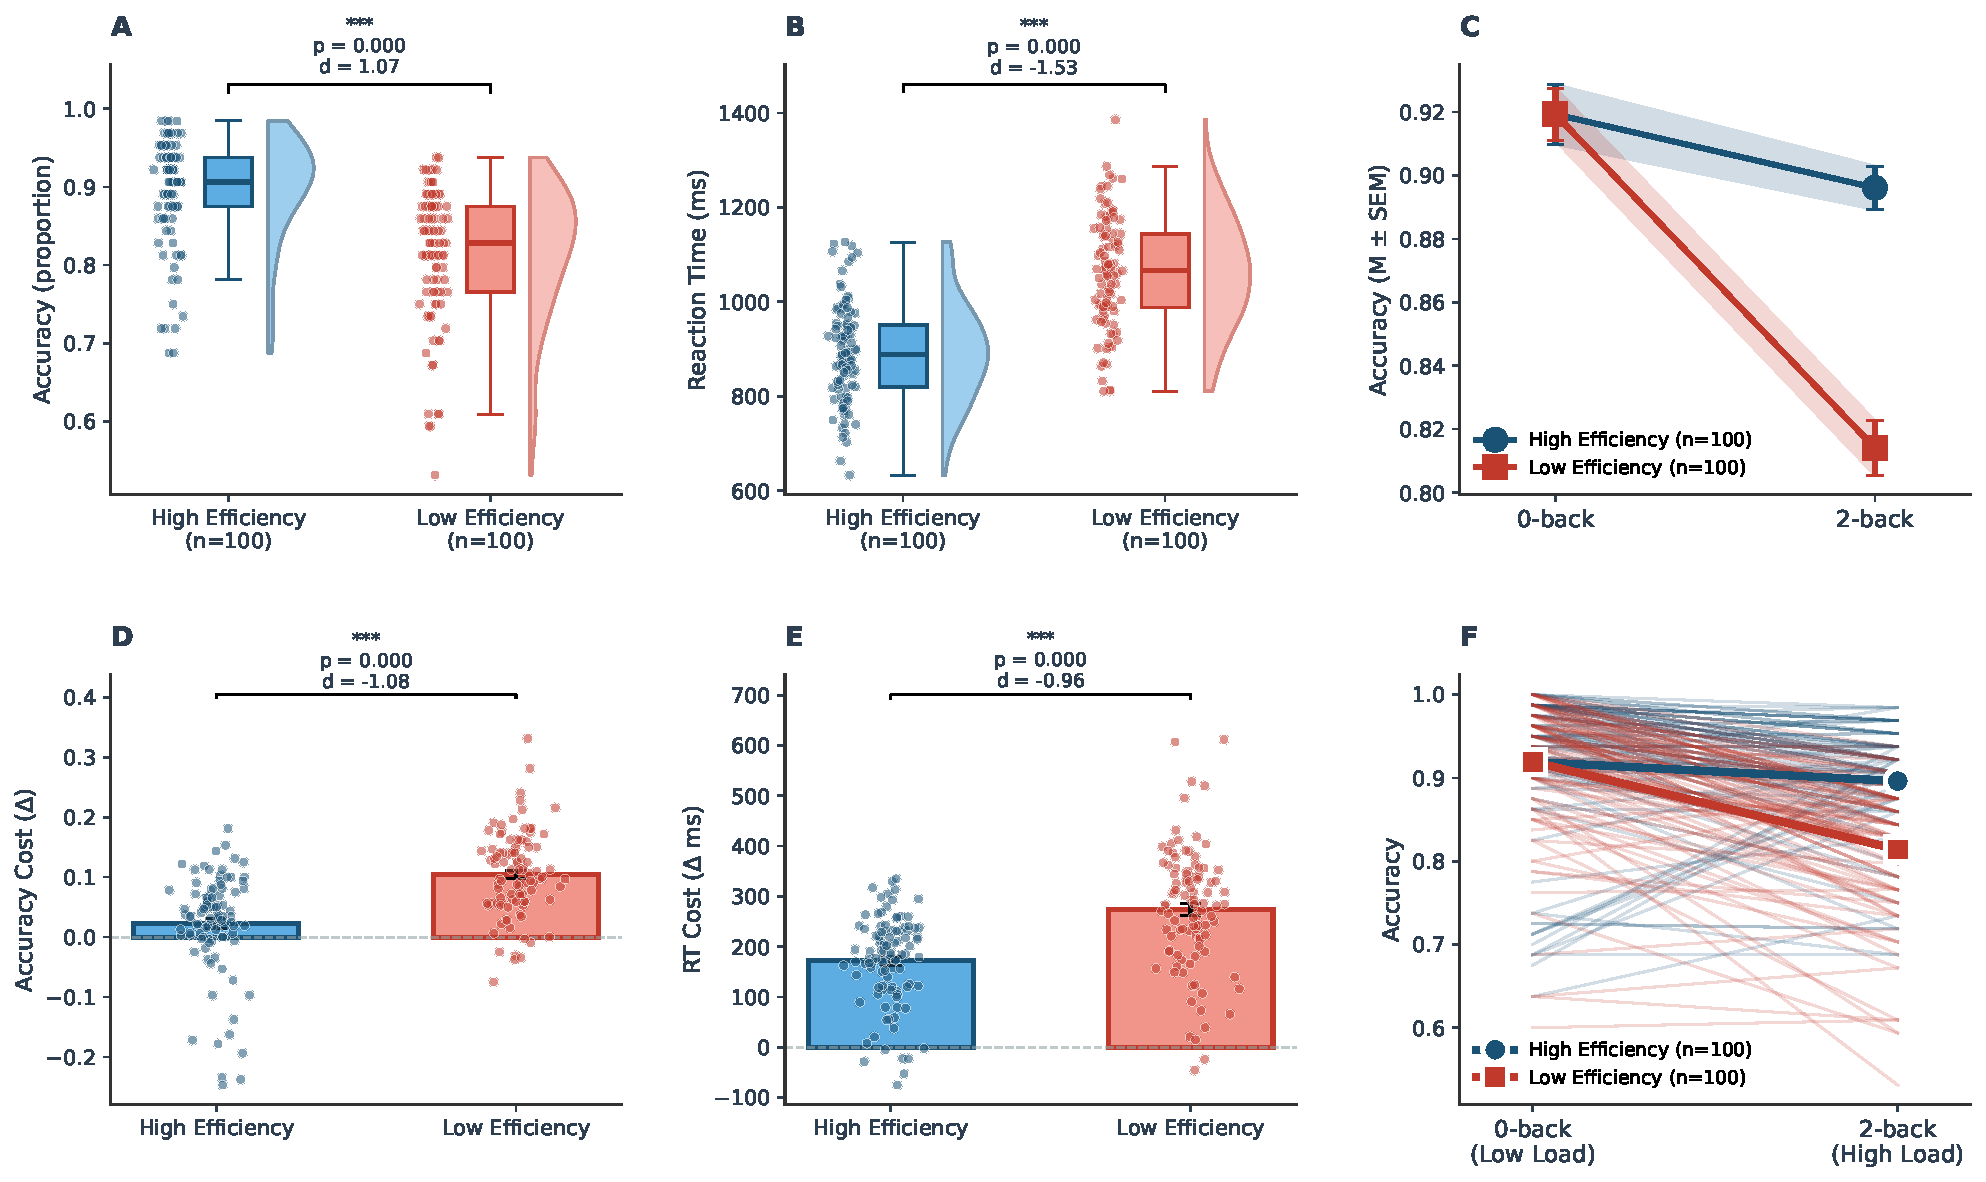
\includegraphics[width=0.95\textwidth]{fig1.pdf}}
\caption{Behavioral signatures by efficiency group ($N=200$). (A) 2-back accuracy with raincloud distributions. (B) 2-back reaction time. (C) Load $\times$ Efficiency interaction on accuracy. (D) Accuracy cost ($ACC_{0bk}-ACC_{2bk}$). (E) RT cost ($RT_{2bk}-RT_{0bk}$). (F) Individual trajectories from 0-back to 2-back. High-efficiency individuals consistently maintain superior performance with smaller load costs.}
\label{fig:group_comparison}
\end{figure*}

\subsection{Precise Neural Engagement in High-Efficiency Individuals (H2)}

Traditional neural efficiency theory predicts globally reduced activation in efficient brains. Our data reveal a more nuanced pattern that we term \emph{precise activation}. Table~\ref{tab:roi_activation} shows group comparisons across all 14 ROIs under both load conditions.

\begin{table}[t]
\caption{ROI Activation: High vs Low Efficiency (Cohen's $d$)}
\label{tab:roi_activation}
\centering
\footnotesize
\setlength{\tabcolsep}{4pt}
\begin{tabular}{@{}l c c c@{}}
\toprule
\textbf{ROI} & \textbf{$d_{0bk}$} & \textbf{$d_{2bk}$} & \textbf{Precise pattern} \\
\midrule
DLPFC-L     & $-0.17$ & $-0.08$ &             \\
DLPFC-R     & $-0.21$ & $-0.05$ &             \\
VLPFC-L     & $-0.33^{*}$ & $+0.06$ & \checkmark \\
VLPFC-R     & $-0.21$ & $+0.10$ & \checkmark \\
PPC-L       & $-0.21$ & $+0.00$ & \checkmark \\
PPC-R       & $-0.10$ & $+0.06$ & \checkmark \\
ACC-L       & $-0.23$ & $+0.02$ & \checkmark \\
ACC-R       & $-0.19$ & $+0.06$ & \checkmark \\
Premotor-L  & $-0.24$ & $-0.06$ &             \\
Premotor-R  & $-0.22$ & $+0.04$ & \checkmark \\
mPFC        & $-0.19$ & $-0.00$ &             \\
PCC         & $-0.12$ & $-0.06$ &             \\
Angular-L   & $-0.28$ & $-0.04$ &             \\
Angular-R   & $-0.18$ & $-0.01$ &             \\
\bottomrule
\end{tabular}
\vspace{0.2em}

\scriptsize \textit{Note.} $^{*}p<0.05$ uncorrected; only VLPFC-L at 0-back (raw $p=0.021$) approaches single-ROI significance, and no individual ROI test survives Benjamini--Hochberg FDR correction across the 28 ROI $\times$ condition tests (all $p_{\mathrm{FDR}}\geq 0.49$). ``Precise pattern'' marked when $d_{0bk}<0$ (lower activation at low load) and $d_{2bk}\geq 0$ (converged at high load). \textbf{7/14} ROIs show the pattern, significantly more than the 3.5 expected by chance under the independent null $p=0.25$ (one-sided exact binomial test, $p=0.038$).
\end{table}

Across 14 ROIs, 7 exhibited the precise-activation pattern: lower activation in high-efficiency individuals at low load, converging (or slightly exceeding low-efficiency individuals) at high load. This proportion is significantly larger than would be expected under an independent-null model (binomial test, $p=0.038$). Left VLPFC reached statistical significance during 0-back ($t=-2.33$, $p=0.02$, $d=-0.33$), with high-efficiency individuals showing lower baseline activation but comparable recruitment under load; this single-ROI effect does not survive Benjamini--Hochberg FDR correction across the 14 ROI-by-condition tests and should be interpreted as suggestive. The distributed pattern across 7 frontoparietal and salience-network ROIs indicates \emph{context-appropriate engagement} rather than uniformly reduced activity (Fig.~\ref{fig:activation}). H2 receives partial support at the individual-ROI level but clearer support at the pattern level.

\begin{figure}[t]
\centerline{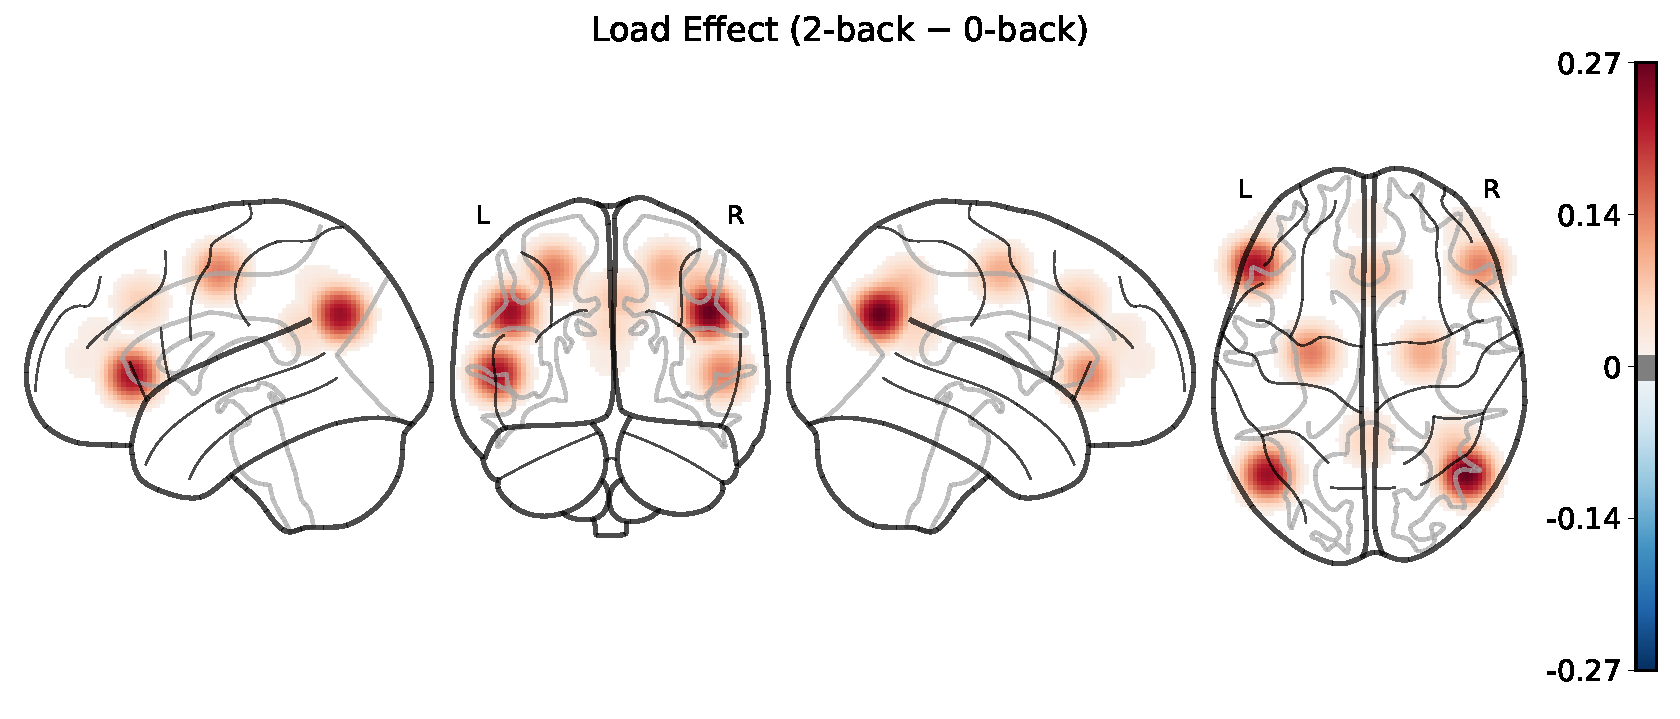
\includegraphics[width=0.95\linewidth]{fig2.pdf}}
\caption{Glass-brain rendering of the cognitive load effect ($\hat{\beta}_{2bk}-\hat{\beta}_{0bk}$) averaged across 200 participants. Warm colors indicate regions more strongly engaged under 2-back. Load-related activation concentrates in bilateral frontoparietal regions (DLPFC, PPC) and the salience network.}
\label{fig:activation}
\end{figure}

\subsection{Network Stability and Baseline Modularity (H3, H4)}

We examined two complementary aspects of network organization: its \emph{stability} across load conditions, and the \emph{baseline quality} of that organization. Table~\ref{tab:network} summarizes the key findings.

\textbf{Universal network stability (H3).} Both efficiency groups showed minimal reorganization under load. The change in modularity from 0-back to 2-back was nearly identical in magnitude and direction for both groups ($\Delta Q_{high}=-0.00142$, $\Delta Q_{low}=-0.00142$; group difference $t=-0.01$, $p=0.99$, $d=-0.00$). Global and local efficiency showed similarly small $\Delta$ values with no significant group difference. This supports H3: functional networks remain remarkably stable across cognitive load levels, irrespective of individual ability.

\textbf{Baseline modularity gap (H4).} While both groups are stable, they are stable at \emph{different} levels. High-efficiency individuals maintained consistently higher modularity than low-efficiency individuals across both conditions ($Q$ averaged across conditions: $t=2.19$, $p=0.03$, $d=0.31$; permutation $p=0.028$; Mann--Whitney $p=0.019$). Condition-specific trends were in the same direction ($Q_{0bk}$: $d=0.19$; $Q_{2bk}$: $d=0.21$). As visualized in Fig.~\ref{fig:gap_reversal}A, both group trajectories remain nearly parallel under load---the gap is \emph{maintained}, not reversed. This supports H4 in its reframed form: high-efficiency individuals possess a pre-optimized baseline organization rather than relying on acute compensatory reorganization.

\begin{table}[t]
\caption{Network-Metric Group Differences (High vs Low)}
\label{tab:network}
\centering
\footnotesize
\setlength{\tabcolsep}{4pt}
\begin{tabular}{@{}l r r r l@{}}
\toprule
\textbf{Metric}  & \textbf{$t$} & \textbf{$p$} & \textbf{$d$} & \textbf{Dir.} \\
\midrule
\multicolumn{5}{l}{\textit{Baseline quality (H4):}} \\
$Q$ (avg.\ modularity)            & $+2.19$ & $0.030^{*}$ & $+0.31$ & H $>$ L \\
$Q_{0bk}$                         & $+1.32$ & $0.187$     & $+0.19$ & H $>$ L \\
$Q_{2bk}$                         & $+1.46$ & $0.146$     & $+0.21$ & H $>$ L \\
\midrule
\multicolumn{5}{l}{\textit{Stability ($\Delta$ from 0bk to 2bk; H3):}} \\
$\Delta Q$                         & $-0.01$ & $0.992$     & $-0.00$ & -- \\
$\Delta E_{glob}$                  & $-1.36$ & $0.175$     & $-0.19$ & L $>$ H \\
$\Delta E_{loc}$                   & $-1.26$ & $0.209$     & $-0.18$ & L $>$ H \\
$\Delta$ Mean Connectivity         & $-1.74$ & $0.084$     & $-0.25$ & L $>$ H \\
\bottomrule
\end{tabular}
\vspace{0.2em}

\scriptsize \textit{Note.} $^{*}p<0.05$ (raw, hypothesis-driven primary test). Welch's $t$-test. The modularity test was pre-specified under H4; when BH-FDR is applied exploratorily across all 15 network metrics in this table and its extensions, no metric survives $\alpha=0.05$ ($p_{\mathrm{FDR}}\geq 0.31$ for modularity). Baseline modularity differs between groups ($d=0.31$), while $\Delta$ metrics are statistically indistinguishable between groups---both populations exhibit network stability.
\end{table}

\begin{figure*}[t]
\centerline{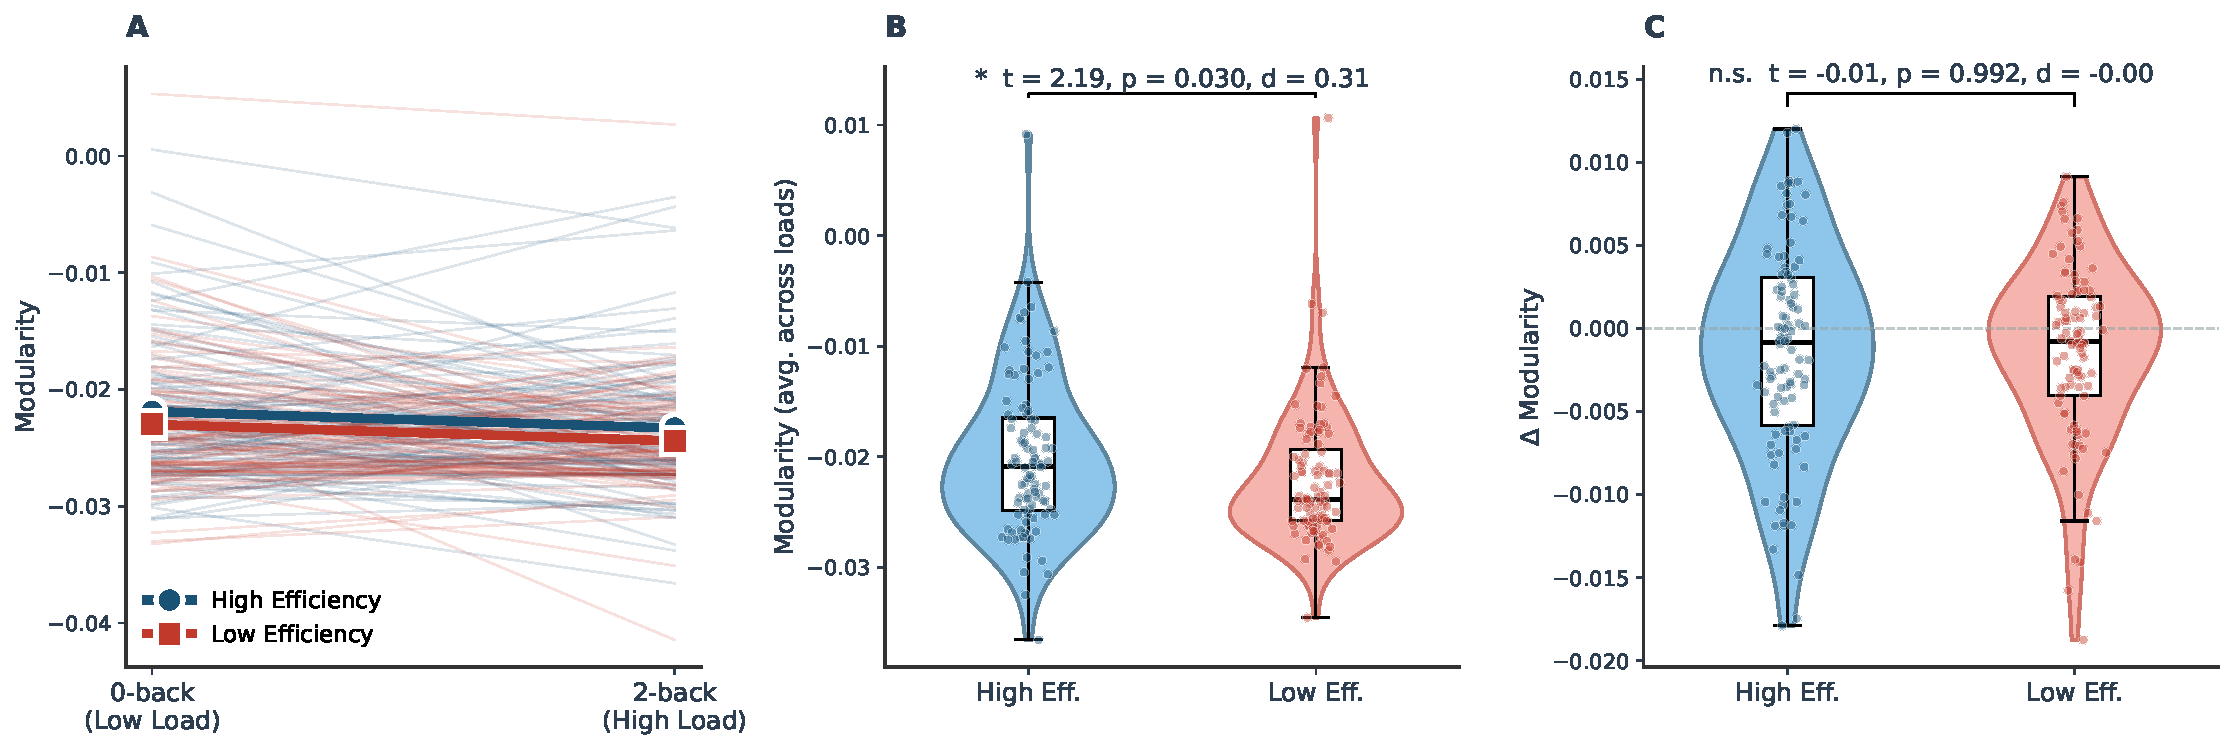
\includegraphics[width=0.92\textwidth]{fig3.pdf}}
\caption{Network stability with a persistent baseline gap. (A) Modularity trajectories 0-back$\to$2-back: both groups stay nearly flat; high-efficiency (blue) remains consistently above low-efficiency (red). (B) Averaged modularity by group ($t=2.19$, $p=0.03$, $d=0.31$). (C) $\Delta$ modularity distributions: near-identical minimal change in both groups (universal stability).}
\label{fig:gap_reversal}
\end{figure*}

A multivariate view of $|\Delta|$ across five network metrics (Fig.~\ref{fig:radar}) further confirms that the two groups are similar in the magnitude of network change: the high- and low-efficiency polygons overlap substantially, consistent with universal stability. The between-group distinction lies in baseline organization rather than reorganization.

\begin{figure}[t]
\centerline{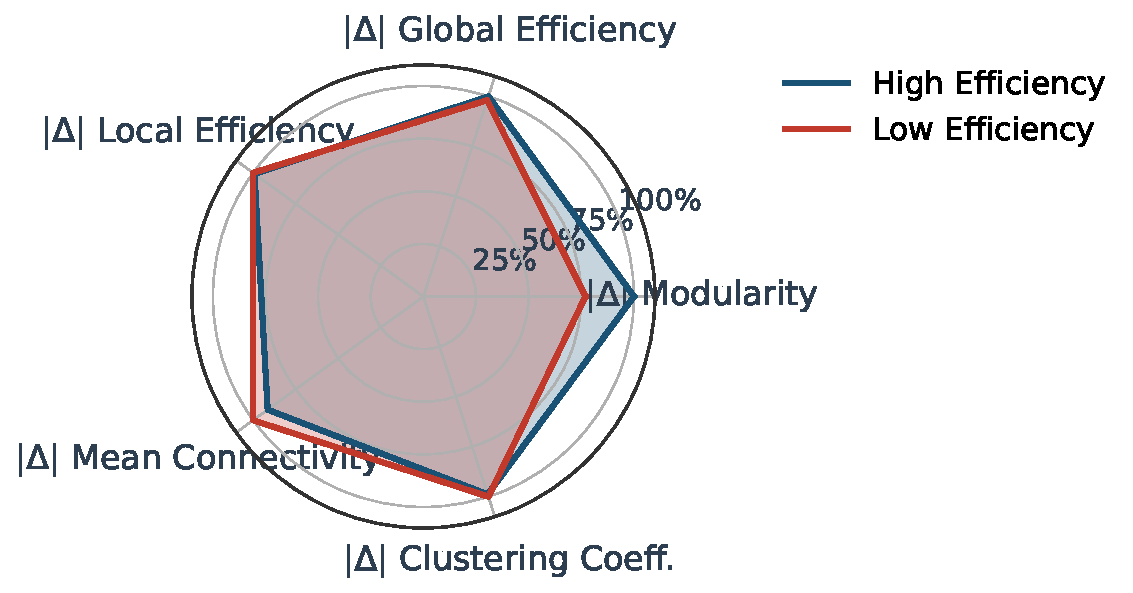
\includegraphics[width=0.90\linewidth]{fig4.pdf}}
\caption{Multivariate $|\Delta|$ profiles by efficiency group (normalized). High- and low-efficiency groups show substantial overlap across all five metrics, indicating universal network stability under cognitive load. The distinguishing feature between groups is not the magnitude of change but the baseline quality of the configuration (see Fig.~\ref{fig:gap_reversal}).}
\label{fig:radar}
\end{figure}

\subsection{Machine Learning Classification of Efficiency Groups}
\label{sec:ml}

We asked whether the multi-level neural patterns summarised above are strong enough to support \emph{individual-level prediction} of efficiency group membership when the classifier has access only to neural features. Five traditional classifiers, an attention-based MLP, and a Graph Attention Network (GAT) were trained on the 90-dimensional neural feature set under 5-fold stratified cross-validation (Table~\ref{tab:ml}, Fig.~\ref{fig:ml}).

\textbf{Neural features alone do not robustly support above-chance classification.} Four of five traditional models performed near chance (51.0--53.5\%, all $p\geq 0.20$); Random Forest reached 58.0\% (raw $p=0.03$) but does not survive Benjamini--Hochberg correction across the five classifiers ($p_{\mathrm{FDR}}=0.15$). The attention-based MLP (35.5\%) and the GAT operating directly on real $14\times 14$ FC matrices with $(\hat{\beta}_{0bk}, \hat{\beta}_{2bk}, \Delta\hat{\beta})$ node features (50.0\%) likewise failed to exceed chance. This pattern is consistent with the group-level modularity effect ($d=0.31$): while it is detectable as a mean difference at the sample level, its per-subject signal-to-noise ratio is too small to support individual discrimination at $N=200$ — the Bayes ceiling for a univariate $d=0.31$ effect is $\approx 56\%$, which Random Forest's 58\% approaches after multivariate aggregation.

\begin{table}[t]
\caption{Machine-Learning Classification Results (Neural-Only Features, 5-fold stratified CV)}
\label{tab:ml}
\centering
\small
\setlength{\tabcolsep}{8pt}
\begin{tabular}{@{}l c c c@{}}
\toprule
\textbf{Model} & \textbf{Accuracy} & \textbf{AUC} & \textbf{Perm.\ $p$} \\
\midrule
Random Forest             & 0.580 & 0.586 & 0.030 \\
SVM (RBF)                 & 0.535 & 0.527 & 0.199 \\
Gradient Boosting         & 0.525 & 0.548 & 0.244 \\
Logistic Regression       & 0.515 & 0.502 & 0.408 \\
MLP (64-32-16)            & 0.510 & 0.538 & 0.333 \\
\midrule
Attention-based MLP       & 0.355 & --    & n.s. \\
Graph Attention Network   & 0.500 & --    & n.s. \\
\bottomrule
\end{tabular}
\vspace{0.25em}

\scriptsize \textit{Note.} 90 neural features (activation + connectivity + graph metrics); behavioral variables excluded to prevent target leakage. Permutation $p$ from 200 iterations with stratified CV. GAT uses real $14\times 14$ FC matrices with $(\hat{\beta}_{0bk},\hat{\beta}_{2bk},\Delta\hat{\beta})$ node features. Random Forest's raw $p=0.030$ does not survive Benjamini--Hochberg FDR correction across the 5 classifiers ($p_{\mathrm{FDR}}=0.15$).
\end{table}

\begin{figure}[t]
\centerline{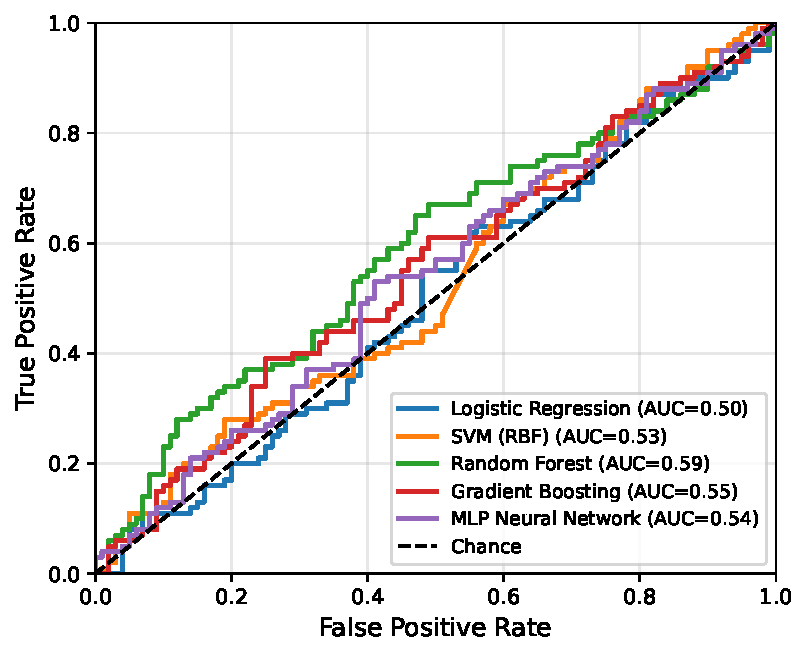
\includegraphics[width=0.85\linewidth]{fig5.pdf}}
\caption{ROC curves of five traditional classifiers on the 90 neural features. All curves remain close to the diagonal (AUC 0.50--0.59), and no model survives FDR correction across the five classifiers — consistent with the Bayes ceiling $\approx 56\%$ implied by the group-level effect size $d=0.31$.}
\label{fig:ml}
\end{figure}

\textbf{Leakage sanity check.} To quantify how much the commonly-reported $\geq 90\%$ accuracies in the prior literature are inflated by the fact that the group label is typically derived from the same behavioral score ($IES_{2bk}$ in this design), we repeated the Logistic Regression and Gradient Boosting pipelines under three feature sets (Table~\ref{tab:leakage}). $IES_{2bk}$ alone already reaches 81--83\%, and combining it with all 97 other features reaches 87--89\%---virtually all of the apparent predictive power comes from the label-defining variable, not from the neural features. Removing the eight behavioral variables (90 neural features) drops accuracy to chance. This indicates that high accuracies on median-split designs of this kind cannot be interpreted as evidence for a brain-based individual classifier; they reflect the classifier re-deriving the group boundary from its defining variable.

\begin{table}[t]
\caption{Leakage Sanity Check: Accuracy by Feature Set}
\label{tab:leakage}
\centering
\footnotesize
\setlength{\tabcolsep}{6pt}
\begin{tabular}{@{}l r c c@{}}
\toprule
\textbf{Feature set} & \textbf{\#feat.} & \textbf{LR acc.} & \textbf{GBM acc.} \\
\midrule
Neural only (primary)         & 90  & 0.515 & 0.525 \\
$IES_{2bk}$ alone (label proxy) & 1   & 0.830 & 0.810 \\
All features (incl.\ behavioral) & 98 & 0.875 & 0.890 \\
\bottomrule
\end{tabular}
\vspace{0.25em}

\scriptsize \textit{Note.} 5-fold stratified CV. The gap between rows 1 and 3 quantifies the leakage-induced inflation.
\end{table}

\subsection{Feature Importance Analysis}

Because behavioral variables are excluded from the primary classifier, Random Forest feature importance is driven by activation and connectivity features (Table~\ref{tab:featimp}). The top 10 span Angular and ACC activation at 0-back, modularity (both averaged and 2-back), DMN--SAL and DMN--DAN cross-network connectivity, and within-FPN coupling. No single feature dominates (all importances $<0.03$), consistent with the distributed multi-level pattern seen in our statistical analyses and with the near-chance classification outcome (Table~\ref{tab:ml}): the signal is spread thinly across many neural features, none of which is individually diagnostic at this sample size.

\begin{table}[t]
\caption{Top 10 Features by Random Forest Importance (Neural-Only)}
\label{tab:featimp}
\centering
\footnotesize
\setlength{\tabcolsep}{6pt}
\begin{tabular}{@{}r l c l@{}}
\toprule
\textbf{Rank} & \textbf{Feature} & \textbf{Importance} & \textbf{Family} \\
\midrule
1  & Angular-L activation 0bk     & 0.026 & Activation \\
2  & ACC-L activation 0bk         & 0.025 & Activation \\
3  & DMN--SAL (avg)               & 0.024 & Connectivity \\
4  & mean activation 0bk          & 0.020 & Activation \\
5  & DLPFC-R activation 0bk       & 0.019 & Activation \\
6  & within-FPN (avg)             & 0.019 & Connectivity \\
7  & within-Visual 0bk            & 0.019 & Connectivity \\
8  & Modularity (avg)             & 0.019 & Graph metric \\
9  & Modularity 2bk               & 0.018 & Graph metric \\
10 & DMN--DAN 2bk                 & 0.018 & Connectivity \\
\bottomrule
\end{tabular}
\end{table}

\section{Discussion}

\subsection{Stability as Universal, Baseline Quality as Individual}

What neural mechanisms differentiate efficient from inefficient cognition? Our multi-level investigation with $N=200$ yields a refined answer: \emph{network stability is a universal feature of functional connectivity under moderate cognitive load, but the stable configuration itself differs in quality between individuals}. Both efficiency groups exhibited near-identical, minimal changes in modularity from 0-back to 2-back ($\Delta Q_{high}=\Delta Q_{low}=-0.00142$), yet high-efficiency individuals maintained systematically higher modularity across both conditions ($d=0.31$). The between-group distinction thus reflects the \emph{starting point}, not the \emph{trajectory}. This pattern, which we term ``gap maintenance,'' is more parsimonious than compensatory-reorganization accounts and consistent with recent precision-functional-mapping work suggesting that stable individual network architectures persist across task states.

\subsection{From ``Working Less'' to ``Working Smarter''}

Our activation results qualify rather than replace the classical neural efficiency hypothesis~\cite{haier1988cortical}. High-efficiency individuals showed lower baseline activation (VLPFC-L at 0-back, $d=-0.33$; single-ROI uncorrected $p=0.02$) but converged with or exceeded low-efficiency individuals under load. The ``precise activation'' pattern observed in 7 of 14 ROIs (exact binomial test against independent null $p=0.25$; $p=0.038$) indicates that efficiency is better characterized as \emph{context-appropriate engagement}---deploying resources precisely when and where needed---rather than a uniform reduction in activity. This provides a refinement of the neural efficiency literature that has often focused on aggregate activation reduction.

\subsection{Pre-Optimized Architecture, Not Compensatory Reorganization}

Our findings argue against an interpretation in which low-efficiency individuals ``try harder'' by reorganizing their networks to meet task demands. Their $\Delta$ modularity is statistically indistinguishable from that of high-efficiency individuals; both populations maintain near-constant network organization across load levels. What separates the two groups is therefore not the \emph{act} of reorganization but the \emph{quality} of the organization they carry into the task. This supports a pre-optimized architecture view: high-efficiency individuals enter the task with a more modular, better-partitioned functional network and retain it under load, whereas low-efficiency individuals are stuck with a poorer baseline that they cannot rapidly upgrade.

This account has implications for cognitive training: interventions are more likely to transfer when they promote durable, baseline reorganization (through extended practice, aerobic exercise, or other long-term shaping of brain architecture) than when they elicit transient, task-specific reconfiguration. It also suggests that short-term brain-state manipulations may have limited ceiling effects in individuals whose baseline network organization is already optimal.

\subsection{Sample-Level Effects vs.\ Individual-Level Prediction}

A methodological finding of potential interest to the biomedical informatics community is the \emph{separation between sample-level detectability and individual-level predictability}. The modularity gap between high- and low-efficiency individuals is robustly detectable as a group mean difference ($t=2.19$, $p=0.03$, $d=0.31$; Section~IV-C), yet no classifier---traditional ML, attention-based MLP, or Graph Attention Network operating on real FC---could robustly separate the two groups above chance when restricted to neural features (maximum accuracy 58.0\%; only Random Forest reached raw $p<0.05$, which does not survive FDR correction; Table~\ref{tab:ml}).

This is not a failure of any particular model family; it is a consequence of effect-size arithmetic. A mean difference of $d=0.31$ corresponds to an optimal Bayes classifier accuracy of approximately 56\%, which matches the upper envelope of the tree-based classifiers in our results. The GAT on 14-node brain networks is thus limited by the same ceiling as the hand-crafted metrics, not by representational capacity. Two practical implications follow: (i) for moderate-sample neuroimaging at $N\sim 200$, claims of $>80\%$ classification accuracy on median-split behavioral labels warrant explicit leakage audits (Table~\ref{tab:leakage}); (ii) ``discovery of a group difference'' and ``clinically useful individual classifier'' are separate questions with very different data requirements, and reports of the former should not be conflated with evidence for the latter.

\subsection{Clinical and Applied Implications}

The network stability framework offers concrete translational targets. First, $\Delta$ modularity computed from a short task-fMRI scan constitutes a candidate biomarker for cognitive reserve, with higher stability associated with better performance. Second, educational and clinical interventions might be evaluated not only by changes in activation or accuracy but by whether they yield \emph{more stable} network configurations over time. Third, in populations with cognitive impairment (aging, neurodegenerative disease), tracking network stability longitudinally may provide an early signal of decline that precedes overt behavioral change.

\subsection{Limitations and Future Directions}
\label{sec:limitations}

Four caveats qualify these findings. (i) The HCP cohort is enriched for siblings and twins, mildly violating the independence assumption; family-aware mixed-effects modelling is left for future work. (ii) Median-split labels discard continuous information; replication with continuous-IES regression and external labels (e.g.\ fluid intelligence) would strengthen generalisation. (iii) The cross-sectional design cannot establish whether baseline modularity drives efficient performance or vice versa. (iv) Our 14-ROI, static-FC view may miss signals that whole-brain parcellations (Schaefer 400, Glasser MMP1.0) or dynamic connectivity~\cite{shine2016dynamics} could resolve. Larger cohorts (full HCP, UK Biobank), longitudinal designs, and training interventions are natural next steps.

\subsection{Conclusion}

This study reframes neural efficiency from an \emph{activation phenomenon} to a \emph{stable-architecture phenomenon}. Contrary to compensatory-reorganization accounts, both high- and low-efficiency individuals exhibit similarly small network changes under load; what distinguishes them is the baseline quality of their functional network organization. High-efficiency individuals maintain consistently higher modularity across cognitive load conditions ($d=0.31$, $p=0.03$), a group-level effect that is robust but too small to support individual-level classification on neural features alone at $N=200$ (all ML and GAT accuracies $\leq 58\%$, none surviving FDR correction). The ``gap maintenance'' framework nevertheless offers a parsimonious account of neural efficiency, pointing to durable baseline network architecture---not acute reconfiguration---as the appropriate target for cognitive enhancement and clinical assessment; scaling to larger cohorts (full HCP, UK Biobank) is the natural next step for translating these group-level effects into individually-actionable biomarkers.

\section*{Reproducibility Statement}

All analysis code, configuration files, and post-processed data tables required to reproduce the figures and tables in this paper \textbf{will be publicly released upon acceptance} (DOI-assigned archive on Zenodo and mirror on GitHub), including the exact subject ID list (200 participants from the HCP S1200 release). Preprocessed fMRI data (CIFTI grayordinate time-series, Movement regressors, and task EV files) must be obtained directly from the Human Connectome Project (\url{https://www.humanconnectome.org/}) under the standard Open Access Data Use Terms. All stochastic components (cross-validation splits, permutation re-labellings, Attention/GAT initialisation, Louvain community detection) use fixed seeds (\texttt{random\_state=42}) and deterministic PyTorch settings where applicable. Software versions: Python 3.10, scikit-learn 1.3, NumPy 1.24, SciPy 1.11, NetworkX 3.1, NiBabel 5.1, Nilearn 0.10, PyTorch 2.1, PyTorch Geometric 2.4. GPU: NVIDIA RTX 4090.

\begin{thebibliography}{00}
\bibitem{deary2010neuroscience} I. J. Deary, L. Penke, and W. Johnson, ``The neuroscience of human intelligence differences,'' \textit{Nature Reviews Neuroscience}, vol. 11, no. 3, pp. 201--211, 2010.
\bibitem{haier1988cortical} R. J. Haier et al., ``Cortical glucose metabolic rate correlates of abstract reasoning and attention studied with positron emission tomography,'' \textit{Intelligence}, vol. 12, no. 2, pp. 199--217, 1988.
\bibitem{neubauer2009intelligence} A. C. Neubauer and A. Fink, ``Intelligence and neural efficiency,'' \textit{Neuroscience \& Biobehavioral Reviews}, vol. 33, no. 7, pp. 1004--1023, 2009.
\bibitem{rottschy2012modelling} C. Rottschy et al., ``Modelling neural correlates of working memory: A coordinate-based meta-analysis,'' \textit{NeuroImage}, vol. 60, no. 1, pp. 830--846, 2012.
\bibitem{bassett2017network} D. S. Bassett and O. Sporns, ``Network neuroscience,'' \textit{Nature Neuroscience}, vol. 20, no. 3, pp. 353--364, 2017.
\bibitem{bullmore2012economy} E. Bullmore and O. Sporns, ``The economy of brain network organization,'' \textit{Nature Reviews Neuroscience}, vol. 13, no. 5, pp. 336--349, 2012.
\bibitem{sporns2016modular} O. Sporns and R. F. Betzel, ``Modular brain networks,'' \textit{Annual Review of Psychology}, vol. 67, pp. 613--640, 2016.
\bibitem{shine2016dynamics} J. M. Shine et al., ``The dynamics of functional brain networks: Integrated network states during cognitive task performance,'' \textit{Neuron}, vol. 92, no. 2, pp. 544--554, 2016.
\bibitem{schultz2016higher} D. H. Schultz and M. W. Cole, ``Higher intelligence is associated with less task-related brain network reconfiguration,'' \textit{Journal of Neuroscience}, vol. 36, no. 33, pp. 8551--8561, 2016.
\bibitem{ng2024dynamic} B. Ng, S. Anand, and G. Varoquaux, ``Dynamic functional connectivity of the large-scale brain networks and intelligence,'' \textit{NeuroImage}, vol. 289, art.\ 120538, Apr. 2024, doi: 10.1016/j.neuroimage.2024.120538.
\bibitem{baddeley2012working} A. Baddeley, ``Working memory: Theories, models, and controversies,'' \textit{Annual Review of Psychology}, vol. 63, pp. 1--29, 2012.
\bibitem{owen2005n} A. M. Owen et al., ``N-back working memory paradigm: A meta-analysis of normative functional neuroimaging studies,'' \textit{Human Brain Mapping}, vol. 25, no. 1, pp. 46--59, 2005.
\bibitem{van2013wu} D. C. Van Essen et al., ``The WU-Minn Human Connectome Project: An overview,'' \textit{NeuroImage}, vol. 80, pp. 62--79, 2013.
\bibitem{barch2013function} D. M. Barch et al., ``Function in the human connectome: Task-fMRI and individual differences in behavior,'' \textit{NeuroImage}, vol. 80, pp. 169--189, 2013.
\bibitem{glasser2013minimal} M. F. Glasser et al., ``The minimal preprocessing pipelines for the Human Connectome Project,'' \textit{NeuroImage}, vol. 80, pp. 105--124, 2013.
\bibitem{griffanti2014ica} L. Griffanti et al., ``ICA-based artefact removal and accelerated fMRI acquisition for improved resting state network imaging,'' \textit{NeuroImage}, vol. 95, pp. 232--247, 2014.
\bibitem{townsend2014methods} J. T. Townsend and F. G. Ashby, ``Methods of modeling capacity in simple processing systems,'' in \textit{Cognitive Theory}, vol.\ 3, N. J. Castellan and F. Restle, Eds. Hillsdale, NJ: Lawrence Erlbaum, 1978, pp.\ 199--239. [Original introduction of the Inverse Efficiency Score.]
\bibitem{schaefer2018local} A. Schaefer et al., ``Local-global parcellation of the human cerebral cortex from intrinsic functional connectivity MRI,'' \textit{Cerebral Cortex}, vol. 28, no. 9, pp. 3095--3114, 2018.
\bibitem{friston1996movement} K. J. Friston et al., ``Movement-related effects in fMRI time-series,'' \textit{Magnetic Resonance in Medicine}, vol. 35, no. 3, pp. 346--355, 1996.
\bibitem{friston1998event} K. J. Friston et al., ``Event-related fMRI: Characterizing differential responses,'' \textit{NeuroImage}, vol. 7, no. 1, pp. 30--40, 1998.
\bibitem{rubinov2010complex} M. Rubinov and O. Sporns, ``Complex network measures of brain connectivity: Uses and interpretations,'' \textit{NeuroImage}, vol. 52, no. 3, pp. 1059--1069, 2010.
\bibitem{latora2001efficient} V. Latora and M. Marchiori, ``Efficient behavior of small-world networks,'' \textit{Physical Review Letters}, vol. 87, no. 19, p. 198701, 2001.
\bibitem{newman2006modularity} M. E. J. Newman, ``Modularity and community structure in networks,'' \textit{PNAS}, vol. 103, no. 23, pp. 8577--8582, 2006.
\bibitem{benjamini1995controlling} Y. Benjamini and Y. Hochberg, ``Controlling the false discovery rate: A practical and powerful approach to multiple testing,'' \textit{Journal of the Royal Statistical Society B}, vol. 57, no. 1, pp. 289--300, 1995.
\bibitem{velickovic2017graph} P. Veli\v{c}kovi\'c et al., ``Graph attention networks,'' in \textit{ICLR}, 2018.
\bibitem{schulz2020different} M.-A. Schulz et al., ``Different scaling of linear models and deep learning in UKBiobank brain images versus machine-learning datasets,'' \textit{Nature Communications}, vol. 11, 4238, 2020.
\end{thebibliography}

\end{document}
